\chapter{Mission: Bio/Xeno}

\emph{\emph{Bio/Xeno} is a RECON+ mission in which the alliances
  attempt to harvest experimental lifeforms crafted by Dr.~Tokh, some
  of the more dangerous of which have escaped amid the fighting!}

\section{Play Area}
\vspace{-2\parskip}
\noindent\begin{stdminipage}{\linewidth-(2in+1.5em)}
\vspace{0pt}   
\noindent
The Deployment Zones are~6'' areas along the short play area edges.

%There is an Exclusion Zone extending~6'' on either side of the short
%centerline of the play area.

There is an Exclusion Zone extending~6'' on both sides of the short
centerline of the play area (12'' across total) and covering the full
extent between long edges.

Place two Stasis Chambers on the short centerline of the play area and
each 5'' from the center toward a different long edge (10'' apart).

A Network Terminal is placed on the centerline of the play area,
adjacent to a long edge of the play chosen before any deployment
begins by the player with Deployment.

\section{Mission Rules}

The Connect Objective short skill may be applied to Stasis Chambers in
this mission.

\end{stdminipage}
\hfill
\begin{minipage}[t]{2in}\centering
\vspace{4pt}   
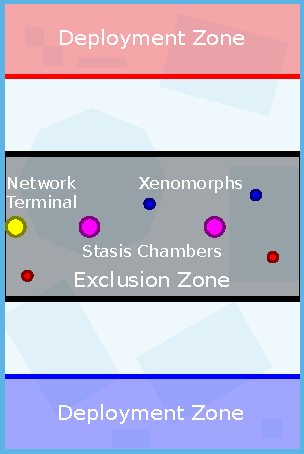
\includegraphics{maps/map-bio}
\end{minipage}

\section{Scoring}

Players may score up to~10 objective points via the following
conditions at game end:
\begin{itemize}\shortlist
\item 1pt for each Console closest to your Deployment Zone connected.
\item 2pts for each Console farthest from your Deployment Zone
  connected.
\item 2pts for having your Special Agent in base contact with a
  connected Console.
\item 1pt if the opposing Special Agent is in a Null state or eliminated.
\item 1pt if more points of the opposing army list have been destroyed.
\end{itemize}

\vfill
\vbox to 0pt{}